\chapter{Results and summary}
\graphicspath{{Chapter5/Figs/}{Chapter5/Figs/}}

This chapter presents the concrete final results, a concise summary of the project in the form of key aspects of a N/CI and an example architecture while considering the initial goals and objectives.

\section{Results}
\label{chapter5-results}

This section discusses the final results of the implementation chapter. The author begins by discussing the most important key aspects and insights of a N/CI for the software components of the NIP for IDUN and then delves deeper into architectural aspects of the technical implementation.

\subsection{Key aspects of a N/CI}
\label{chapter5-key-aspects}

Previously, the author coined the term N/CI within a defined by the three-dimensional axes spanned by production-readiness, general applicability and unobtrusiveness (see \autoref{fig:nci-definition-intro}). However, this illustration does not address the aspects on how to come up with a holistic technological definition. Subsequently, the following subsections discuss some architectural, ethical, and privacy aspects of the exemplary built N/CI for IDUN Technologies.

\subsubsection{Stream-based events}
\label{chapter5-stream-based-events}

One of the most critical technical aspects of a N/CI is the stream-oriented and event-driven architecture. An event-driven architecture is typical in modern applications built with microservices and uses events to trigger and communicate between decoupled services \citep{amazon_web_services_inc_event-driven_nodate}. The stream-oriented aspect describes the main events happening in such a system. Neural data recorded from IDUN's sensors is being streamed from the end-user's devices and processed on the cloud to transform and classify the raw data to generate applicable and intelligible output. There are two main differences between the stream types when building a N/CI:

\begin{enumerate}
  \item \textbf{Synchronous streams} for active and real-time BCI.
  \item \textbf{Asynchronous streams} for passive, reactive BCI.
\end{enumerate}

Either a user streams neural data from the device to the cloud in order to generate actionable insights, such as controlling an object in a game, or the user tries to improve audio amplification based on where they look at. Such use cases necessitate real-time classification within an acceptable latency (more on latency in the following subsection).

The other component occurs when an asynchronous stream is used in place of a synchronous stream. For example, while asleep, the user does not require real-time insights from their sleep. When they wake up, the system must stop the stream, classify it, and display, e.g. the sleep stages. These various aspects are crucial because the data stream is required to undergo some sort of data transformations, such as the calculation of frequency band power (typically done in EEG signal processing). Therefore, there needs to be a specific time window (epoch) to calculate a plausible output. To determine the proportion of, say, alpha waves (which typically have frequencies between 8 and 13 Hz) in a user's neural data, we must decompose the raw EEG signal into frequency components via a fast Fourier transform (FFT). An example of FFT transformed data is visualised in \autoref{fig:fft}.

\begin{figure}[!ht]
  \centering
  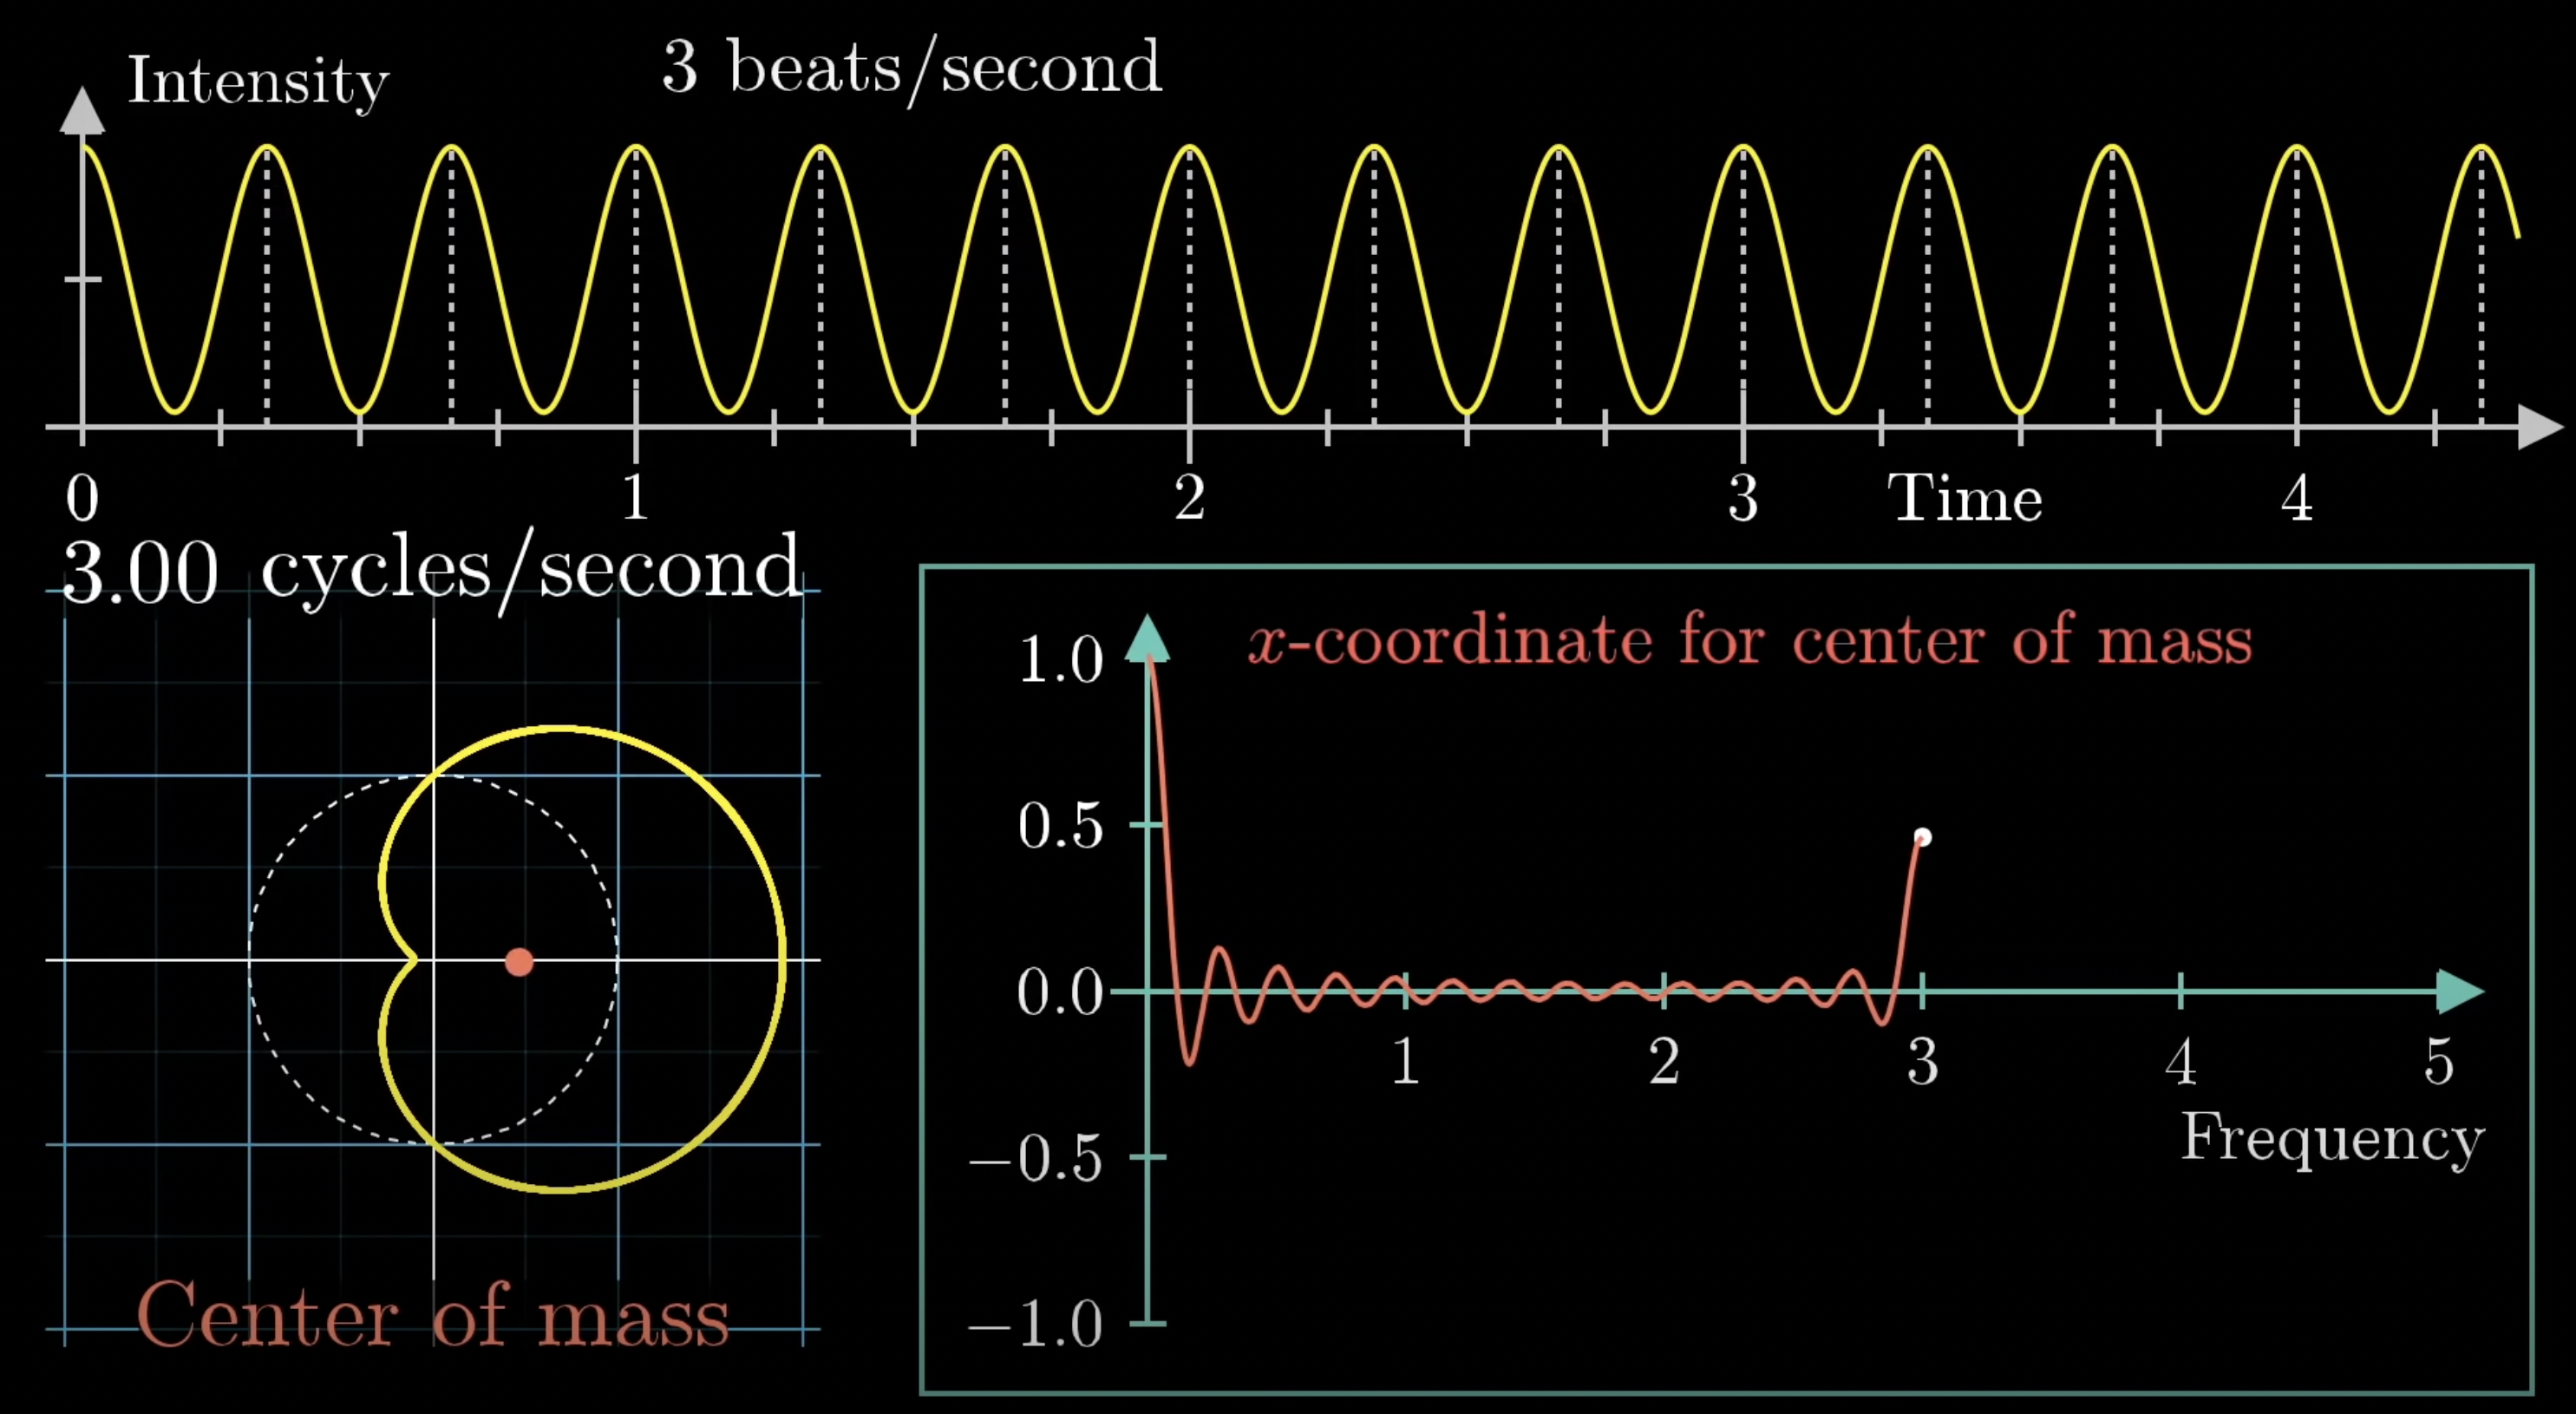
\includegraphics[width=\linewidth]{fft.png}
  \caption[Illustration of how FFT works]{Illustration of how FFT works \citep{3blue1brown_but_2018}}
  \label{fig:fft}
\end{figure}

A given frequency in the time series is used to calculate the cycles to extract the originally occurring frequency signal based on the epoch length. As a result, we have, on the one hand, an epoch-based classification of neural data where the classifier makes prediction based on an epoch-by-epoch sequence. On the other hand, we have a per-sample shift classification where the prediction happens within a buffer that stores a fixed length of historical samples and moves sample-by-sample following a first in first out (FIFO) principle. The latency of per-sample classification is 0.004 seconds (due to the 250 samples of the IDUN sensor) whereas a per-epoch classification initially has a latency of 1 second due to filling up the buffer for e.g. for FFT. \autoref{fig:per-sample} visualises the differences between these stream transformation types.

\begin{figure}[!ht]
  \centering
  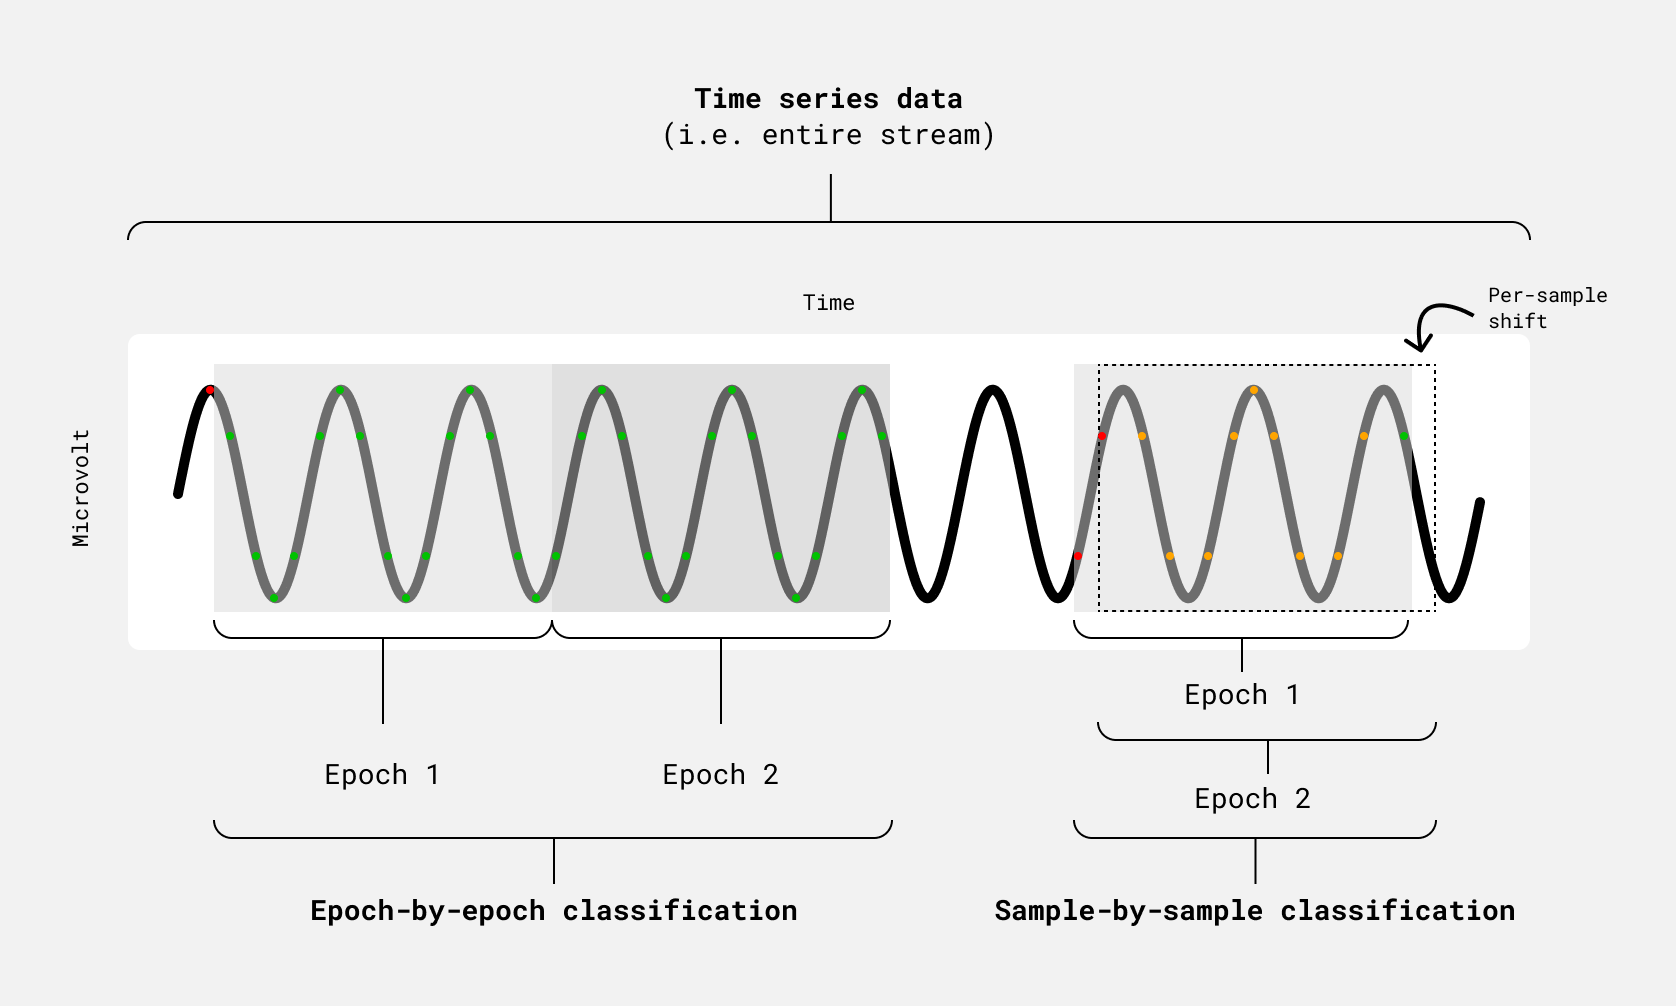
\includegraphics[width=\linewidth]{per-sample.png}
  \caption{Illustration of two real-time classifications for a BCI application.}
  \label{fig:per-sample}
\end{figure}

\subsubsection{Critical and non-critical applications}
\label{chapter5-critical-and-non-critical-applications}

The discussion of stream-based events leads us to the aspect of critical and non-critical use cases. In a critical use case such as microsleep detection, while driving, we need a synchronous neural stream with a low-latency classification of whether the driver is currently awake, asleep or about to fall asleep. In such use cases, the classification needs to be as fast as possible, such as in a sample-by-sample classification, so it is more about how fast the connection between the measuring sensor and the classifier is. In very critical use cases, where, e.g. a user's life may depend on it, the classification would need to be done without an active internet connection so that the classification model runs on the hardware itself and not in the cloud in order to be able to intervene within milliseconds (e.g. in the form of a loud sound to warn or wake up the driver), as a few moments can make the difference between fatalities.

Not-so-critical applications can fall back on online modes and run classifiers over an active internet connection in the cloud. To reduce latency, edge cloud computing could be introduced, where business logic executed in the cloud is brought geographically closer to the end user via edge locations \citep{nomios_what_nodate}. The aspect of edge-cloud or edge-computing in general is a topic that is not covered in the aspects of a N/CI in this thesis since it was not a requirement to build a critical system at IDUN.

However, the distinction between critical and non-critical streams can be made not only for synchronous streams, as described in the preceding examples, but also for asynchronous streams, particularly in the context of research. In general, research represented by, e.g. IDUN's persona Noel does not necessitate synchronous streams or real-time classifications but rather the most reliable possible acquisition of neural data from test subjects. The critical aspect in such a use case can also be much higher than, e.g. recording neural data during sleep in consumer-oriented applications. For example, if the device goes offline or the Bluetooth connection is lost, the device must cache the data locally and be able to restore and send it once the device is back in range or restore a sufficiently stable internet connection. The author recommends having a fallback system in the form of buffering for each data stream, e.g. if neural data becomes corrupted or misordered due to timestamp mismatches in sending the data over the internet. This could mean that a particular EEG sample could arrive earlier than another sample which would have been earlier in the time series. Therefore some sorting algorithm would need to run over the arriving samples as shown on \autoref{fig:sorting}. Luckily, Kinesis already comes built-in with a guaranteed order mechanism via sequence numbers to solve this problem \citep{amazon_web_services_inc_amazon_nodate}.

\begin{figure}[!ht]
  \centering
  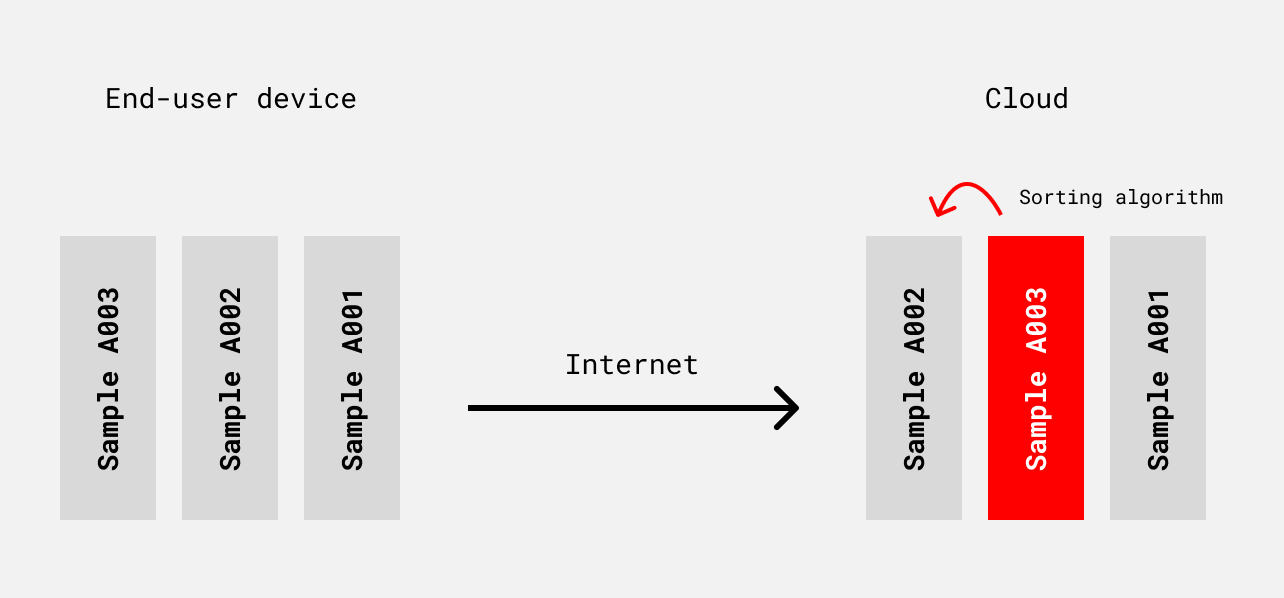
\includegraphics[width=\linewidth]{sorting.png}
  \caption{Mechanism of sorting samples as they might arrive in the wrong order on the cloud via the internet.}
  \label{fig:sorting}
\end{figure}

The other aspect is buffering the data when the device is offline. It periodically sends a health check request to the cloud via WebSocket in a given interval and buffers all data on the interval. If no promise returns after a certain threshold, the device (or SDK on the end-user device) starts to buffer as shown on \autoref{fig:buffering}.

\begin{figure}[!ht]
  \centering
  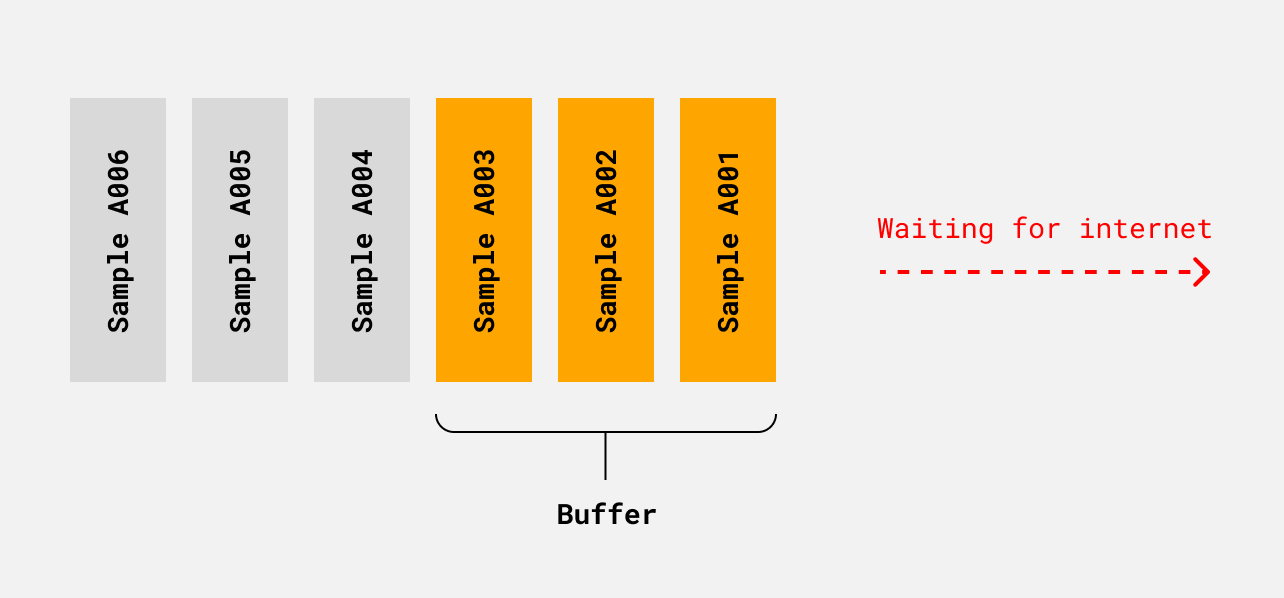
\includegraphics[width=\linewidth]{buffering.png}
  \caption{Buffering mechanism on the device (i.e. end-user device such as a smartphone) when there is no internet connection.}
  \label{fig:buffering}
\end{figure}

\subsubsection{Opt-in and encryption}
\label{chapter5-opt-in-and-encryption}

Because IDUN develops an unobtrusive library (in the form of an SDK, as detailed in \autoref{appendix4-further-implementation-key-events}) that can be easily implemented in existing software such as web apps or mobile apps, the developers of these apps have actual access to the hardware and initiate the Bluetooth connection between the sensor and the end-user device. IDUN must encrypt the recorded data on the hardware before it reaches the third-party app to protect user privacy and the security of end-user neural data.

\begin{figure}[!ht]
  \centering
  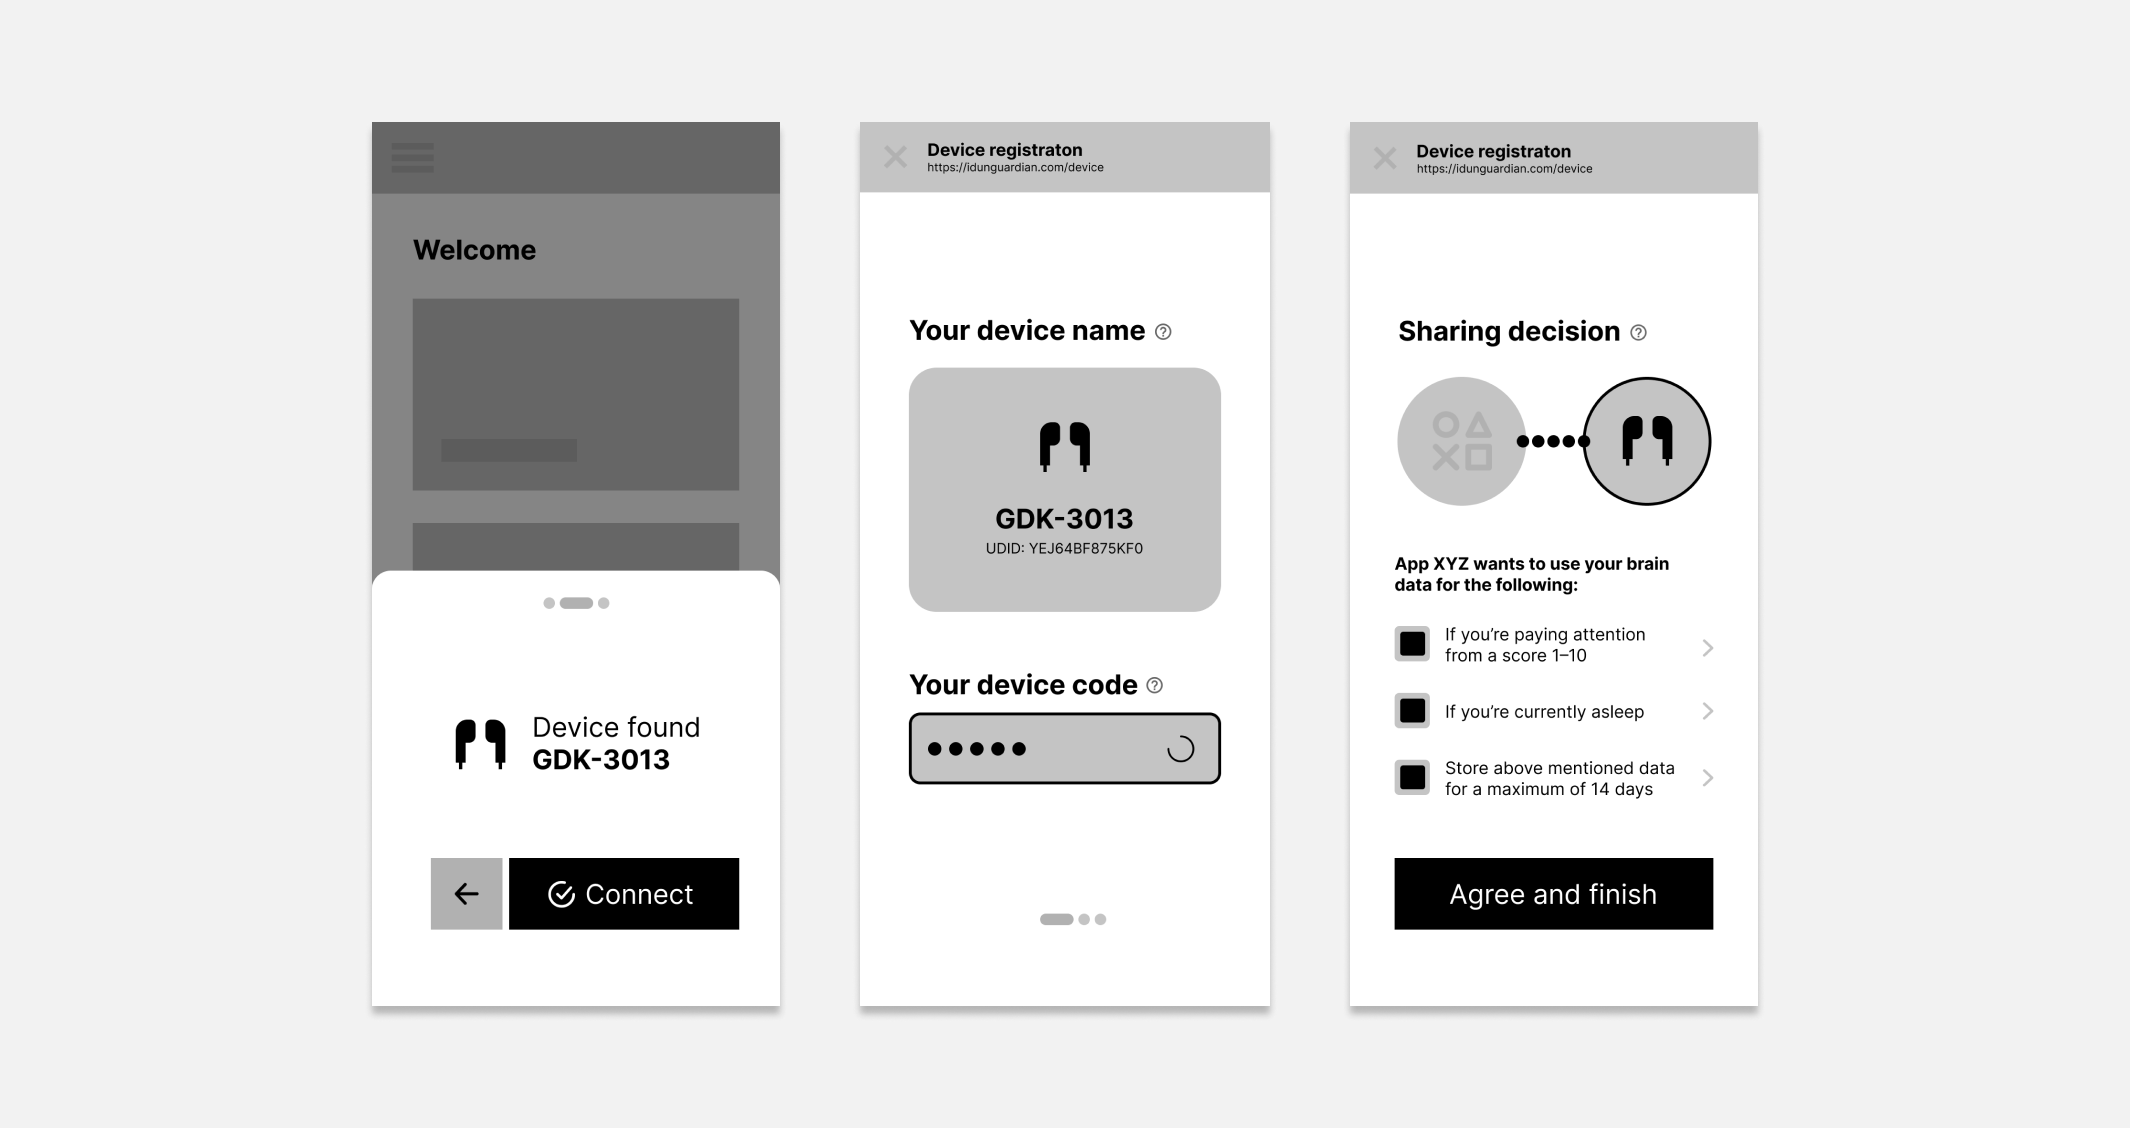
\includegraphics[width=\linewidth]{auth-flow.png}
  \caption{Wireframes for the opt-in mechanism. Starting with the device connection via BLE, the device registration (or login) and then opt-in for app-specific options.}
  \label{fig:auth-flow}
\end{figure}

This is a critical step in preventing third-party providers from collecting extensive data and classifying insights from users they may not want. IDUN securely decrypts the data in its cloud using the private key in the asynchronous encryption example. Third-party developers can thus only access data that the user has authorised. The duration of data storage, the type and level of detail of certain classifications of their neural data, and sharing and usage analysis are all opt-in options. \autoref{fig:auth-flow} depicts how such an opt-in mechanism might appear as a GUI in a third-party mobile app.

Unencrypted raw data should never be accessible to third parties and poses some technical challenges. To visualise and display the raw time series of IDUN's EEG sensors, e.g. the individual display images would have to be rendered on the server and streamed to the client as a video stream. Another difficulty is synchronising and organising the rotation of public and private keys, which must be done without interference from third parties. Asynchronous encryption, together with envelope encryption, is a production-ready and battle-tested method to solve this issue. In envelope encryption, the data key (public key) is itself also encrypted with the private key \citep{google_cloud_envelope_nodate}.

\begin{figure}[!ht]
  \centering
  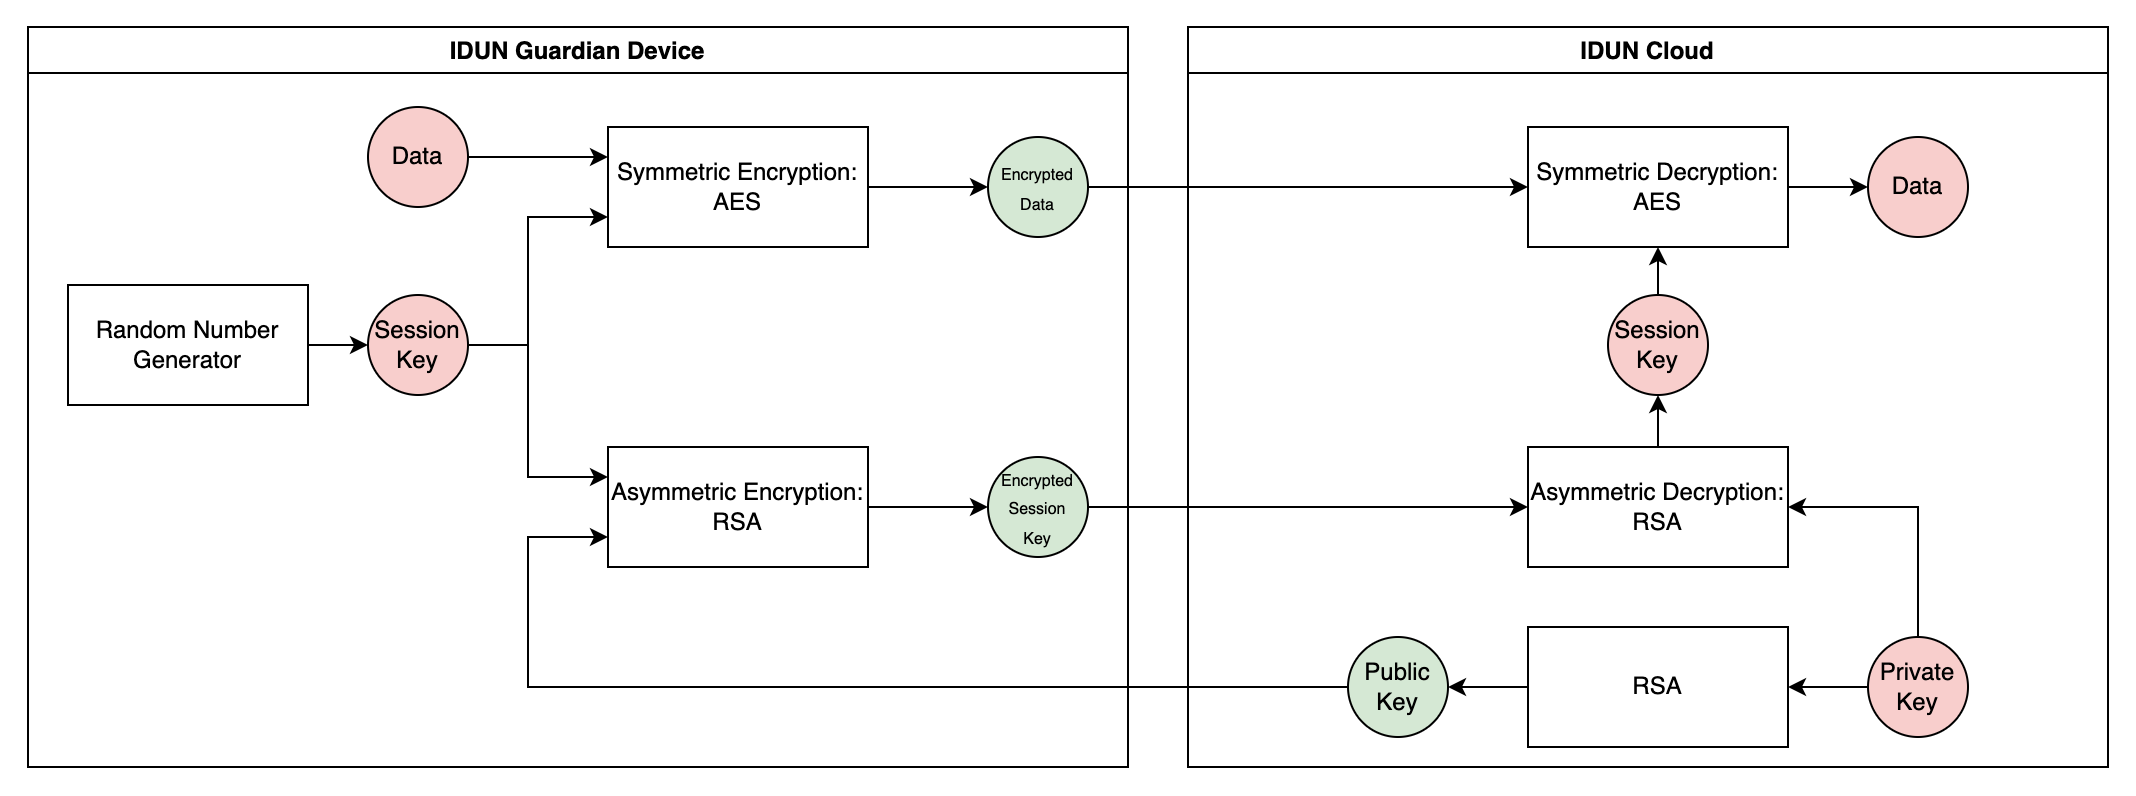
\includegraphics[width=\linewidth]{encryption-model.png}
  \caption[Hybrid encryption model to encrypt and therefore protect the raw EEG data]{Hybrid encryption model to encrypt and therefore protect the raw EEG data \citep{idun_guardian_nodate}.}
  \label{fig:encryption-model}
\end{figure}

\subsubsection{Graph data access}
\label{chapter5-graph-data-access}

Aside from the stream-oriented, event-driven nature of a N/CI, the aspect of data storage is critical. It is important to note that, due to the high frequency of the EEG data, it became apparent during the implementation phase that storing the neural data in a database is not an efficient method. Storing it as a static file on an object storage system like AWS S3 in a text-based file format like comma-separated values (CSV) files seemed more appropriate and scalable since it is too much data for a database. Similar to how other static data such as images get stored on object storage as well, and only the URL to the object is stored in a database rather than storing the entirety of the bytes from the image inside the database \citep{datanamic_store_nodate}.

In addition to storing the neural data in the given data structure, it is essential to note that other sensor data, such as inertial measurement unit (IMU) data, which is also collected by the IDUN hardware to track the subject's three-dimensional location, rotation, and movement, is also stored alongside and synchronised with the neural data. In addition to the two time-series-based data, EEG and IMU, IDUN collects meta-information such as classified versions of the data, such as eye movement data, which must also be synchronised with the raw data streams. The more classification and post-processing logic applied to raw data streams, the more metadata and relationships must be linked to the original file, as \autoref{fig:graph-database} shows.

\begin{figure}[!ht]
  \centering
  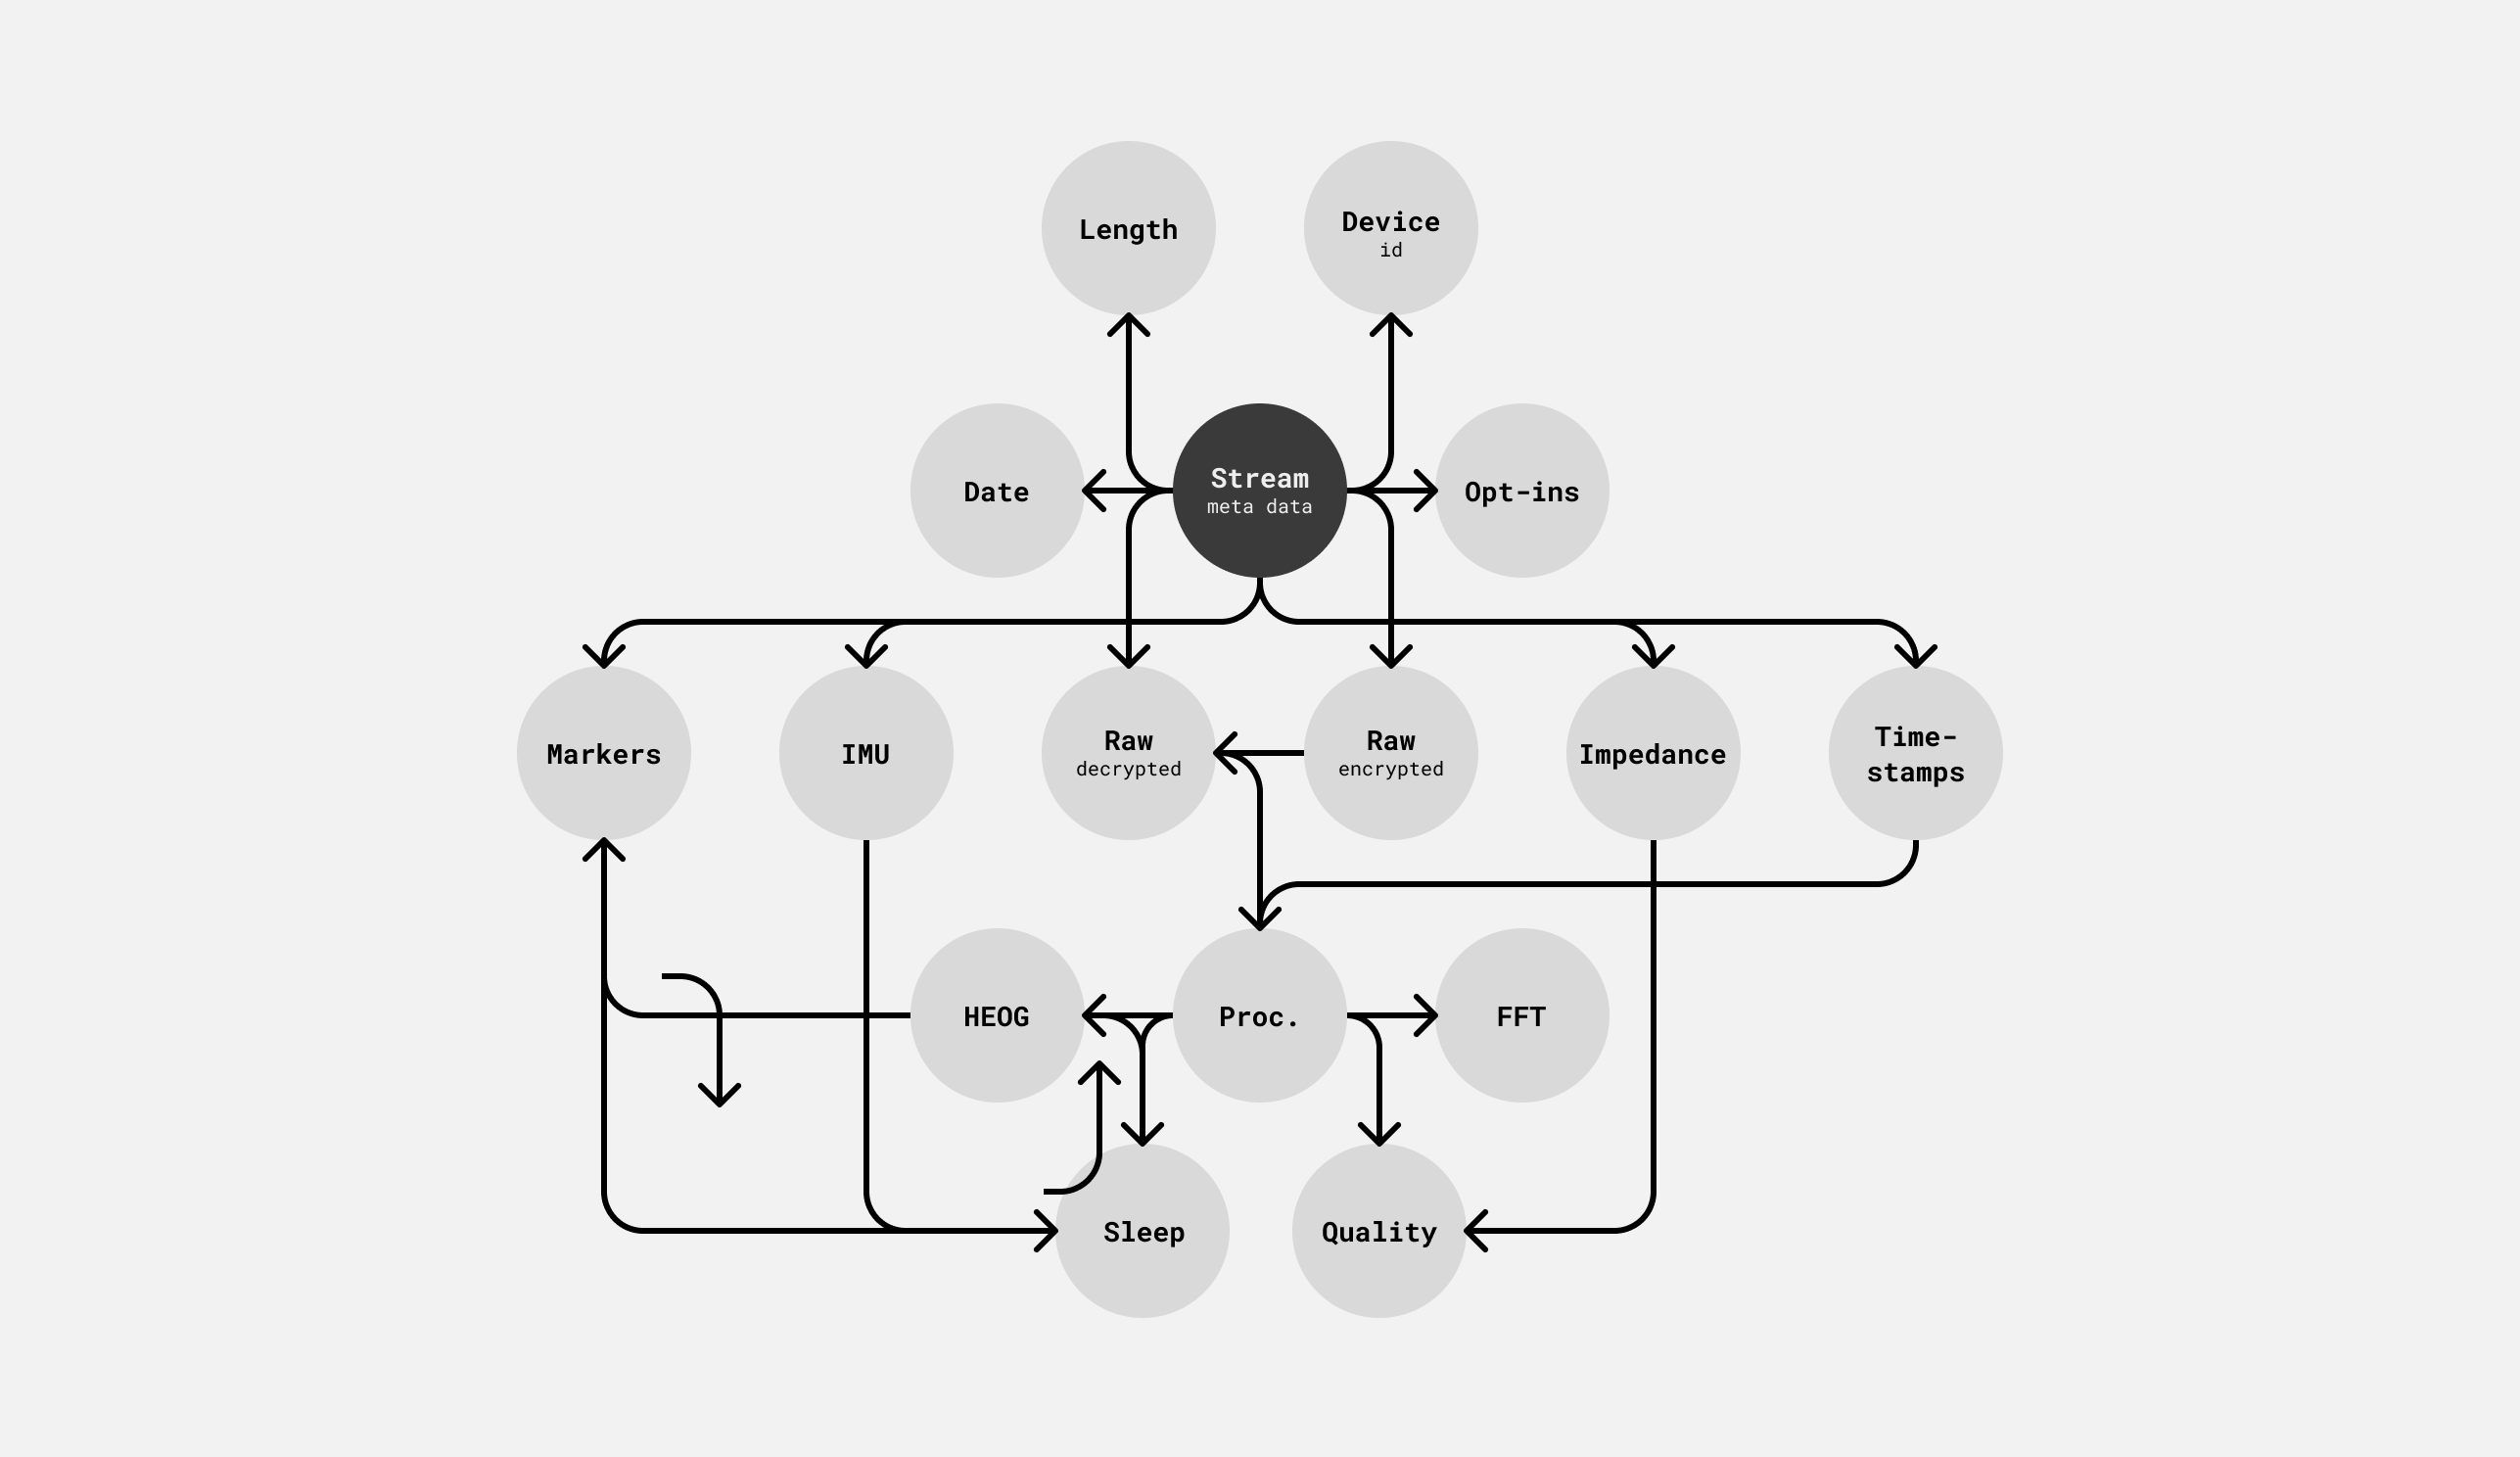
\includegraphics[width=\linewidth]{graph-database.png}
  \caption{Data model in the form of a graph with the current setup and scope.}
  \label{fig:graph-database}
\end{figure}

A graph database is the most natural way to store this large number of relationships between various stored files (entities). Relationships are treated as first-class citizens in graph databases, and most of their value is derived from these relationships. In graph databases, nodes are used to store data entities, while edges are used to store relationships between entities \citep{amazon_web_services_inc_what_nodate}. Due to time limitations, the author did not implement a graph database but chose a relational database such as AWS Aurora since the current amount of data relationships is still manageable. To quickly swap the underlying database technology without rewriting a significant portion of the business logic, the author intends to use an object-relational mapping (ORM) tool such as Prisma to treat relational data models via a graph-like schema \citep{prisma_data_nodate}.

\subsection{Example architecture of a N/CI}
\label{chapter5-example-architecture-of-a-nci}

Based on the key aspects of the N/CI for IDUN's NIP mentioned in the previous subsection, the author presents as one of the main results the following cloud architecture in \autoref{fig:example-architecture}.

\begin{figure}[!ht]
  \centering
  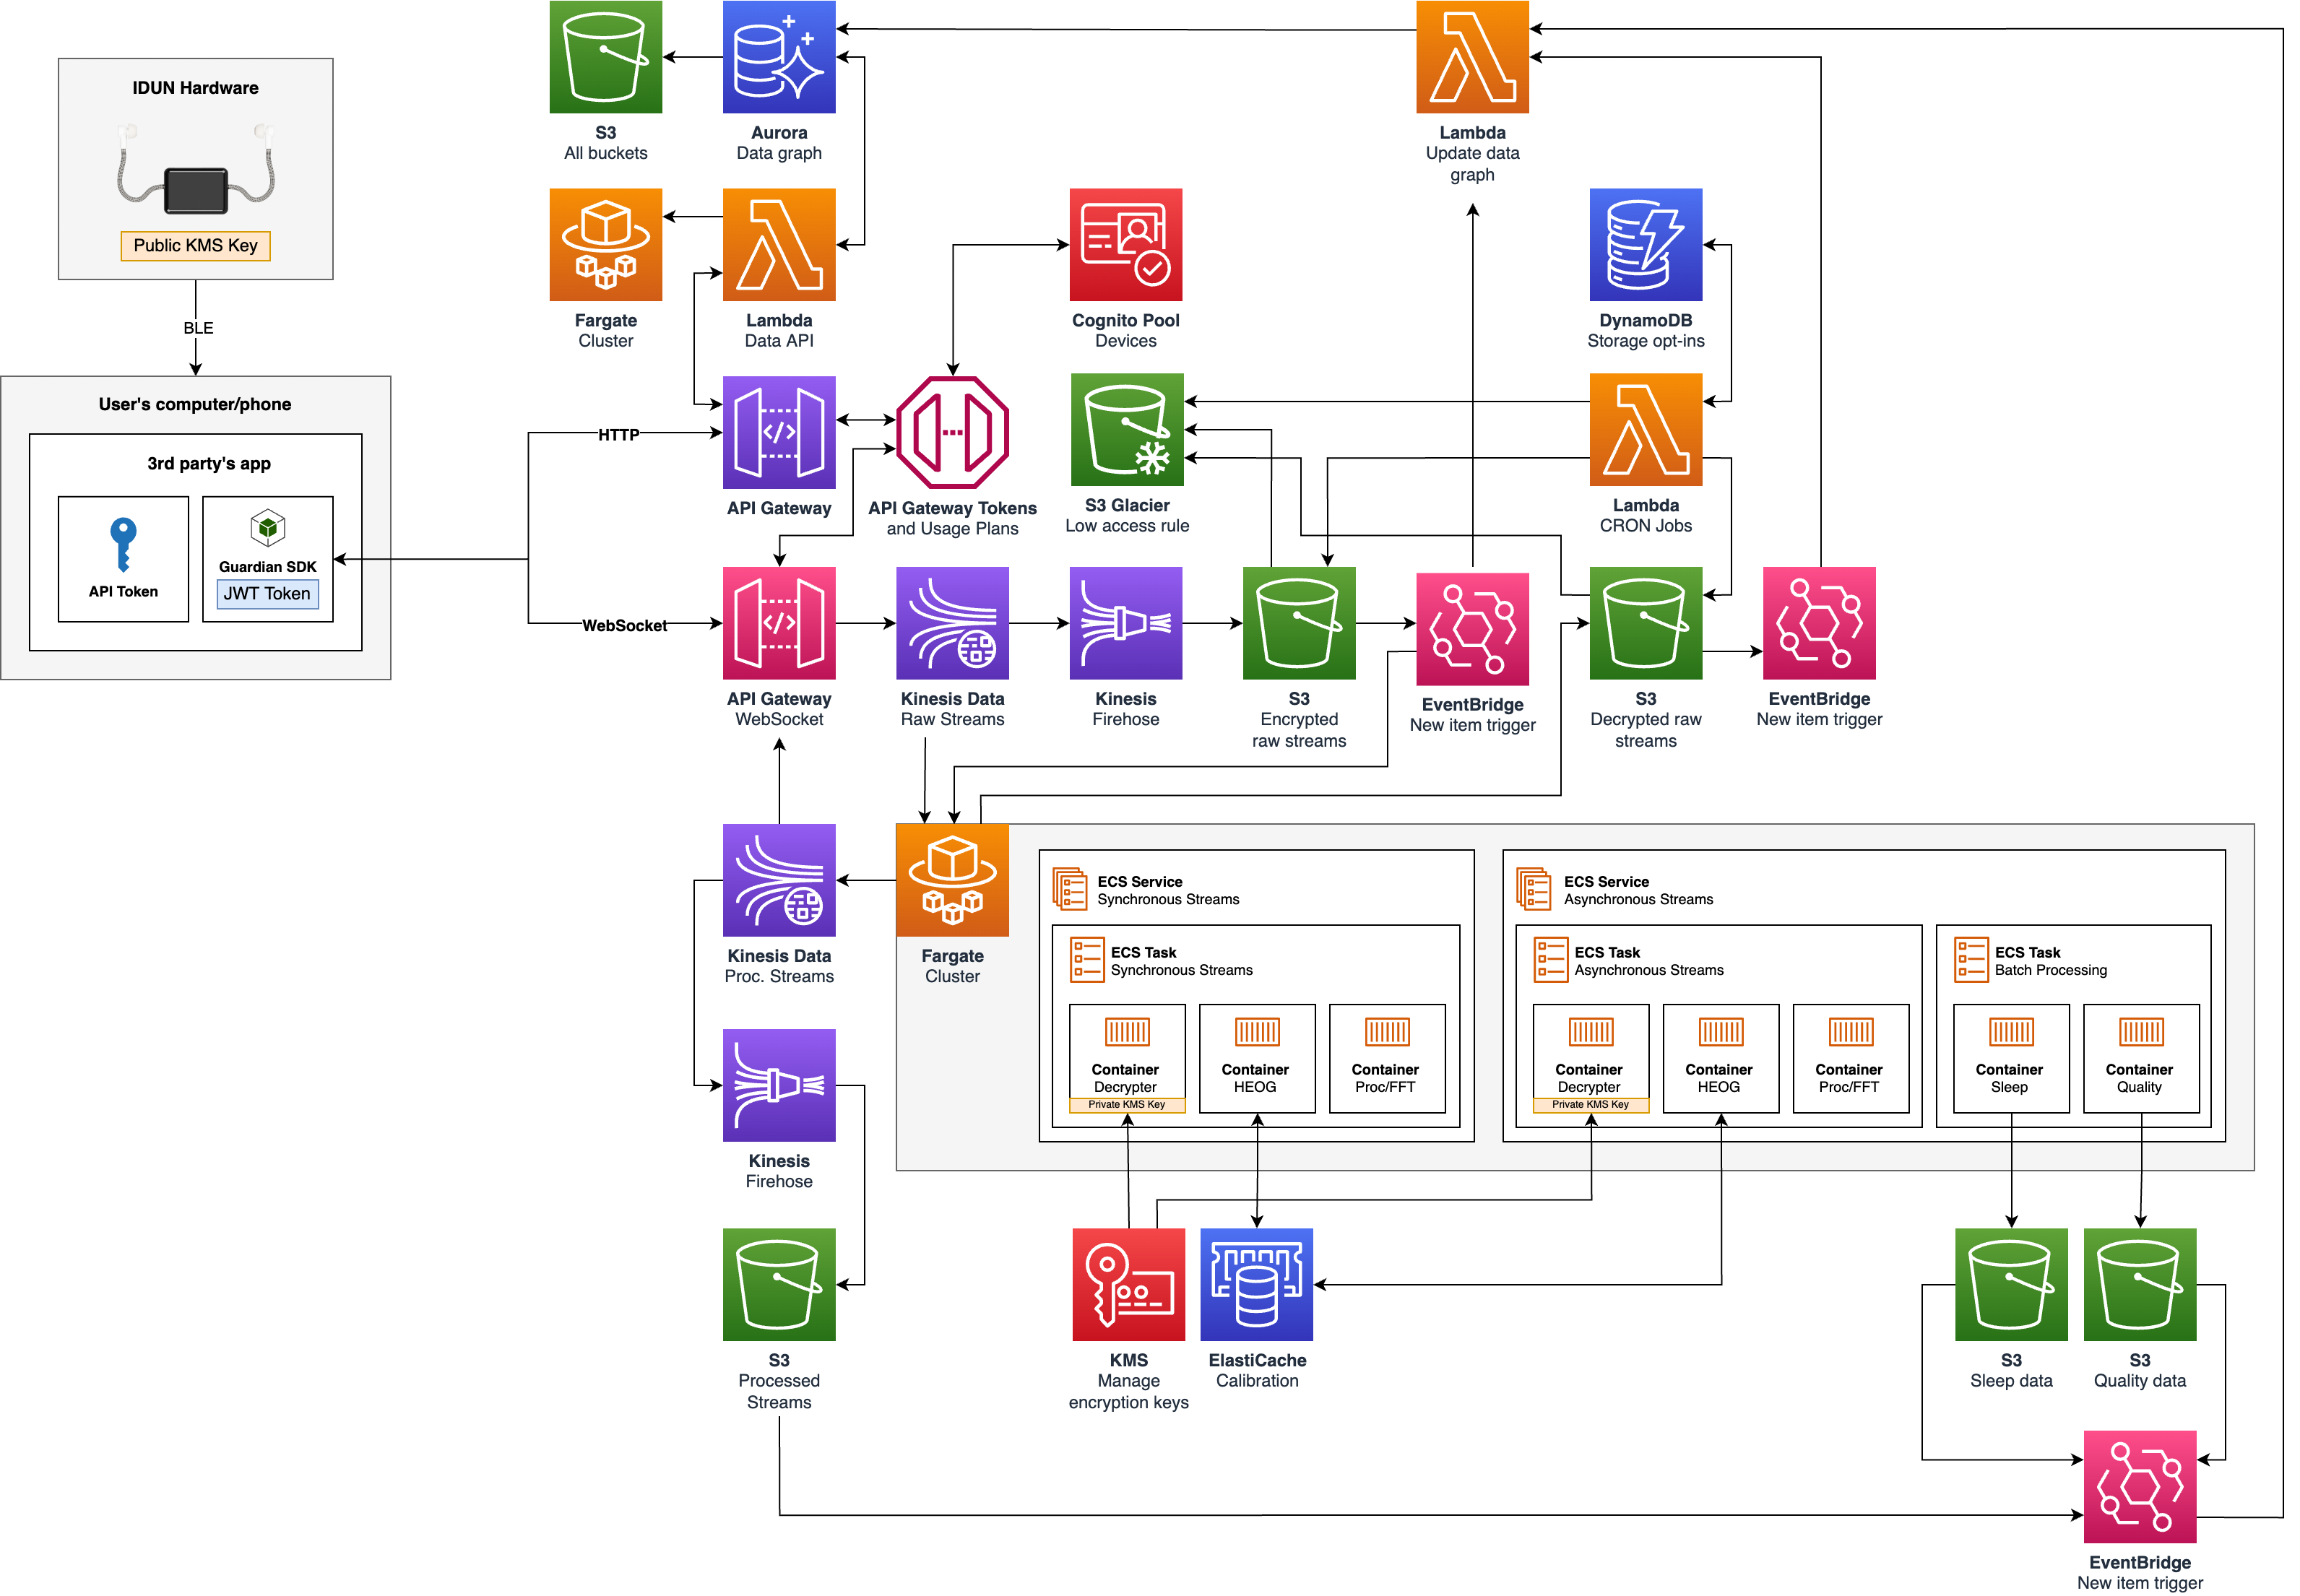
\includegraphics[width=\linewidth]{example-architecture.png}
  \caption{Implementation architecture for IDUN Technologies' N/CI.}
  \label{fig:example-architecture}
\end{figure}

\newpage

The example architecture does not detail the SDK and demo parts described in the user interview insights in \autoref{chapter4-user-interview-insights}. The goal is only to explore the cloud aspects of a N/CI and its core architectural components. The diagram contains some patterns that have specific reasons. The following list describes the different patterns and sections of the mapped architecture and the associated technical descriptions. It is important to note that some parts are not discussed as they are not part of this work, such as the networking aspect of the cloud setup (e.g. virtual private clouds (VPCs), network address translation services (NATs) and security groups and their traffic rules).

\begin{itemize}

  \item \begin{figure}[!ht]
          \centering
          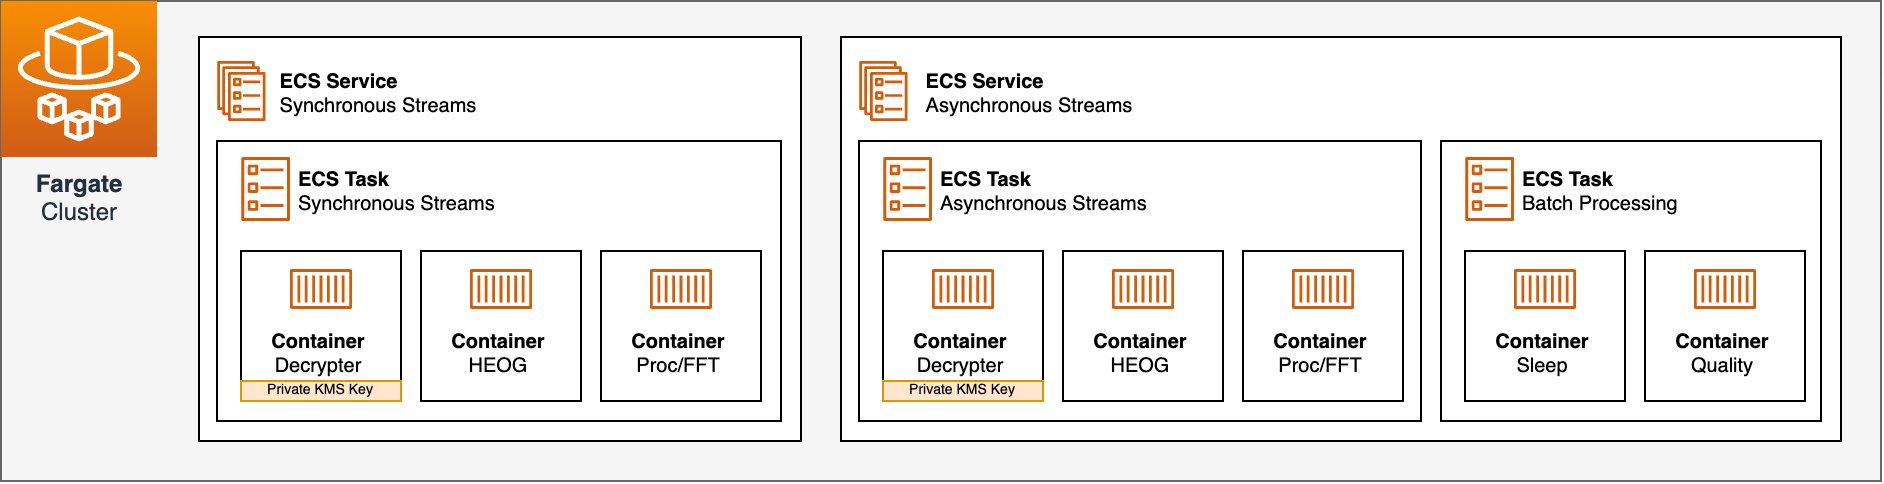
\includegraphics[width=\linewidth]{cluster.png}
          \caption{The Fargate cluster of the example architecture for IDUN's N/CI.}
          \label{fig:cluster}
        \end{figure}

        \autoref{fig:cluster} shows the Fargate cluster of the IDUN cloud setup. There are two primary services: one for business logic applied to synchronous streams and one for asynchronous streams. The distinction can usually be described as the left service being a system of record and the right service being a derived data system \citep{kleppmann_designing_2017}. This separation describes that the system of record processes the raw data directly and, in this case, in a real-time stream, whereas the derived data system generates other data from the raw data without a real-time aspect. There is a certain redundancy, as can be seen, e.g. with the HEOG\footnote{HEOG in this context, which is an acronym for horizontal electrooculogram, and describes the electrical signal recorded to detect the horizontal eye movement.} container (a classifier that recognises in which direction a user is looking). This is due to the aspect of critical and non-critical mentioned earlier. The HEOG container for synchronous tasks runs on a more powerful machine than, for example, the asynchronous container, so their hardware task descriptions differ in available computing power, as the asynchronous neural data processing is not as critical in terms of latency as the synchronous containers.

        Another aspect is that the asynchronous service also contains batch processing containers, e.g. for sleep or general quality classifiers that do not need a stream-based aspect. These classifiers would run on demand or as batch processing events to produce other transformed data not represented as a time series, such as neural data or the other stream-based classifiers. For more information on the decision to use a Fargate cluster, see \autoref{appendix4-further-implementation-key-events}.

        Another important aspect is the decrypted container, which uses the private keys of the key pair to encrypt the data on the hardware and then decrypt it within the services to process and handle the actual and encrypted raw data. When the data is stored in S3 buckets, it is encrypted both in flight and at rest.

  \item  \begin{figure}[!ht]
          \centering
          \hspace*{0.4in}
          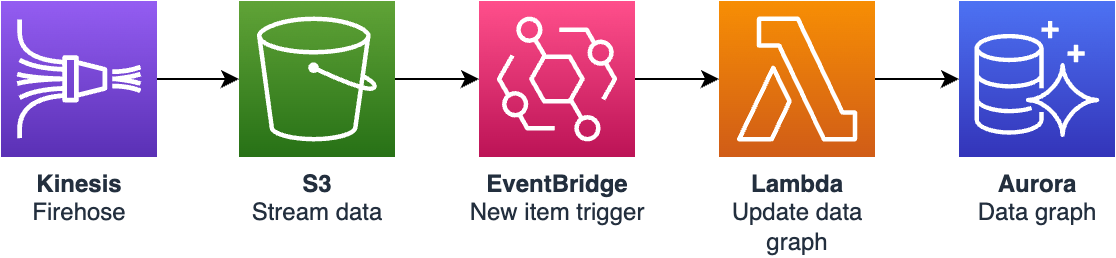
\includegraphics[width=0.9\linewidth]{initial-dataflow.png}
          \caption{The initial data flow in IDUN's N/CI.}
          \label{fig:initial-flow}
        \end{figure}

        \autoref{fig:initial-flow} describes the initial data flow of streamed neural data. The data is sent via the WebSocket protocol to Kinesis, a data ingestion system for data streams. A complimentary service for Kinesis, called Kinesis Firehose, is then used to aggregate the data and store the streamed data as a CSV in an object store, in this case, S3. As more data is streamed through Kinesis, Firehose appends the newly captured data to the CSV file already created on S3. Once the stream is stopped, the CSV file on S3 is marked as complete, which triggers an event in the EventBridge service, which then triggers a Lambda function to add the newly captured file and its meta-information (such as size and identifier) to the data graph database, in this case, the Aurora database service. This event-driven aspect allows the Fargate cluster not to be disturbed and the focus to be on the streaming aspect, with the creation of the data graph being event-driven. In contrast to creating another service in the Fargate cluster, a serverless function in Lambda is not always used to run this business logic because they are event-driven and per-request and thus can be cold rather than hot functions\footnote{Hot and cold functions describe the underlying state of the infrastructure on which business logic is executed on. The serverless aspect of cloud computing functions, such as Lambda, can be "turned off" as soon as the business logic is not needed at the moment, therefore, be described as cold.}, which, e.g. classification logic on the Fargate cluster should always be because people can stream EEG data continuously for hours.

  \item  \begin{figure}[!ht]
          \centering
          \hspace*{0.4in}
          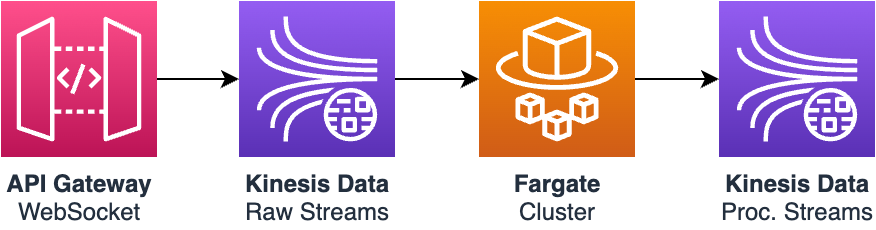
\includegraphics[width=0.8\linewidth]{real-time-dataflow.png}
          \caption{The real-time data flow in IDUN's N/CI.}
          \label{fig:realtime-flow}
        \end{figure}

        \autoref{fig:realtime-flow}, compared to the previous bullet point, shows the real-time data flow. It describes that neural data is sent via the WebSocket protocol and then ends up in the ingestion service of Kinesis. Kinesis stores the data stream and the new incoming data stateful and leaves it to the Fargate cluster to copy and transform the data according to the desired classification, such as HEOG or FFT. Once the Fargate cluster returns the processed or transformed data, it is sent to another Kinesis stream, which then returns the data via the same WebSocket API gateway. As a client, one would only subscribe to one API WebSocket API endpoint in this architecture, although the streams are processed separately with two ingestion services (the Kinesis instances Raw Streams and Proc. Streams), abstracting this logic.

  \item \begin{figure}[!ht]
          \centering
          \hspace*{0.4in}
          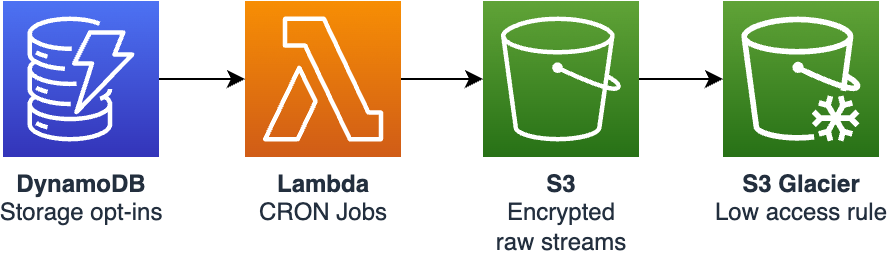
\includegraphics[width=0.8\linewidth]{cron-jobs.png}
          \caption{CRON jobs example architecture in IDUN's N/CI.}
          \label{fig:cron}
        \end{figure}

        \autoref{fig:cron} describes the CRON\footnote{CRON comes from the command line utility that is a job scheduler on Unix-like operating systems to execute tasks repeatedly without human intervention.}. Job processes to process and dictate specific opt-ins from users regarding long-term data storage. Example: If the user has declared that IDUN should not store sleep data in the cloud for longer than four weeks, business logic must check which files are older than four weeks and then delete them. This task of repeatedly checking opt-ins stored in a DynamoDB database can also be handled by a Lambda. DynamoDB is a NoSQL database perfect for data whose schema is challenging to track due to e.g. the complexity of opt-in variations. This business logic can happen four times a day, for example, and has no real-time impact on end users, so this is a good use case for using business logic that can be cold.

        Another aspect is that the CRON Job Lambda defines old files, for example, and places them in cold storage on S3 Glacier. One can transfer old and infrequently used data from warm to cold storage in seconds while the data remains discoverable and searchable \citep{sayed_introducing_2021}. This is a process of removing less frequently used or requested data from the N/CI's computational space, mainly saving cloud costs.

  \item \begin{figure}[!ht]
          \centering
          \hspace*{0.4in}
          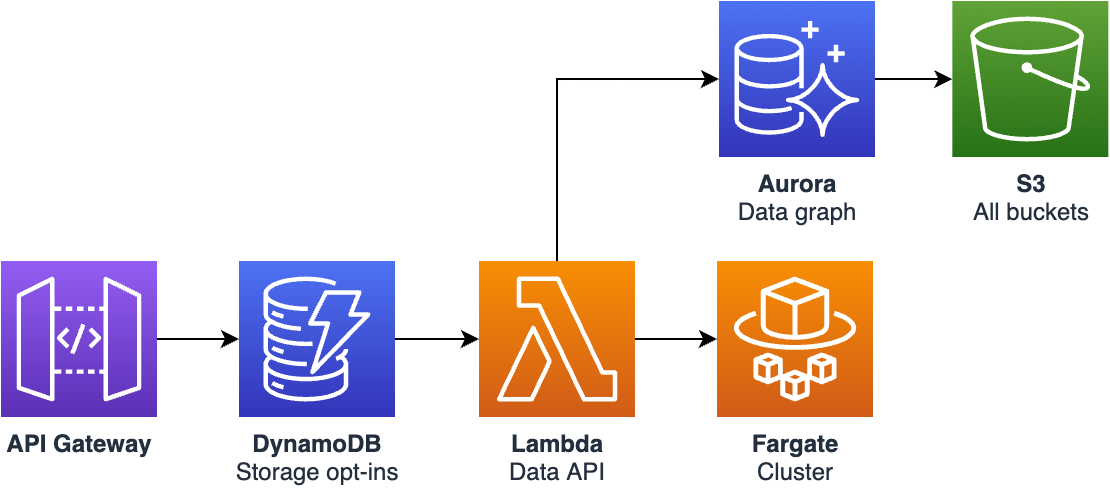
\includegraphics[width=0.8\linewidth]{api-access.png}
          \caption{API access part of the architecture of IDUN's N/CI.}
          \label{fig:api-access}
        \end{figure}

        \autoref{fig:api-access} shows the API access part of the example architecture for IDUN's N/CI. Here the author uses the API Gateway service, not the WebSocket version, but the standard Hypertext Transfer Protocol (HTTP) version, as there is no real-time and stream-based aspect to this API. Based on the opt-in of the users, which is accessible via the API for, e.g. third-party developers, a Lambda accesses the Aurora database, which contains the references to all data stored in S3 buckets within the cloud. For example, if certain data is not available (e.g. if the device is only streaming raw data for, e.g. sleep classification, but the developers want to get the FFT version of the file), then the data API Lambda sends a request to the Fargate cluster to process the data via a batch processing service, as shown in \autoref{fig:cluster}. The updated data is then stored in an S3 bucket directly by Fargate, which triggers another event in EventBridge, as shown in \autoref{fig:initial-flow}, which then updates the data graph. Once the data graph of the specific transformed version of the file has changed, it can be returned as an HTTP response via the API Gateway service.

\end{itemize}

\newpage

\section{Summary}
\label{chapter5-summary}

Within this thesis the author has given the foundational work on the development and the definition of a N/CI. In addition, the author has addressed the challenges and the limitations surrounding the implementation for an exemplary N/CI at IDUN. The given context of working in a fast-moving startup like IDUN did not make the work on the project as well as the written part easy. Nevertheless, the author is satisfied with the result as described in this thesis. The author learned many things ranging from fundamental theoretical neuroscience to cloud computing.

This thesis first has introduced the topics and some of the essential terms and their backgrounds in the introductory chapter in \autoref{chapter1-background} and has concluded from the possibility of the current state of research to the aims and objectives for this thesis.

The assumption that the implementation of a N/CI is feasible with contemporary technologies has been proven but still has its unknown shortcomings that need to be identified. Nevertheless, the aim was to provide the reader with an overview and context of the newly introduced definition of N/CI and the lessons learned during its practical implementation at IDUN. The context and motivation for creating a N/CI, as described as the first item in the list of objectives, were derived in chapter 2 and explained in more detail in \autoref{appendix1-definition-and-motivation-of-a-nci}. Compared to existing systems and research, the clear definition, distinction and advantages of a N/CI were also described in more detail in \autoref{appendix1-definition-and-motivation-of-a-nci}. The identification and definition of key aspects to realise a N/CI to demonstrate general applicability for BCI software were shown using key events in \autoref{chapter4-timeline} and \autoref{chapter5-key-aspects}. The implementation details of an example architecture of a N/CI, which was this thesis's fourth and final objective, were presented in \autoref{chapter5-example-architecture-of-a-nci}. Therefore, the author summarises that all goals and objectives were achieved in this project.

\subsection{Reflection}
\label{chapter5-reflection}

Creating an exemplary N/CI in the industry as part of IDUN Technologies' NIP was a non-trivial and complex undertaking. There were many moving parts and many imponderables. Also, since no other person is publicly building a N/CI or anything that would fall into the definition of a N/CI, the author could not count on experienced engineers who have built such a system for a mass market BCI before. The biggest problem in the context of this work was the sheer scale of the project, as reflected in the length of the paper. In hindsight, it might have been better to focus more precisely on one deliverable rather than having four objectives and primary goals. The author should also have defined more clear criteria for what the work packages should have been and what defines them as finished. The work was more theoretical than initially anticipated and focused on the definition and key aspects of a N/CI, ultimately a by-product of the original work.

\subsection{Outlook}
\label{chapter5-outlook}

The author intends to publish certain parts of this work in the form of a research paper. An exciting part is the definition and motivation behind creating the new discipline in which Neural/Cloud Interfacing resides. In addition, the author will continue to work at IDUN Technologies to develop their N/CI further and document the upcoming technological challenges in the form of, e.g. blog posts.

An important aspect and a change that will occur once IDUN sells its device to the general public is that the currently proposed architecture, as shown in \autoref{chapter5-example-architecture-of-a-nci} is for a localised system, i.e. the cloud data centre is in one geographical location (in IDUN's example: EU-Central-1 in Frankfurt). For example, this aspect could be worked on as part of a possible Master's thesis. As an outlook, a look at a distributed cloud system could be fascinating, as scaling around the world population would require a distributed system to reduce latency and fault tolerance.

\subsection{Conclusion}
\label{chapter5-conclusion}

A N/CI is an essential and new definition of a discipline between cloud computing and BCI software. This new discipline brings many new challenges, such as making a neural interface software system ready for production, which brings layers such as privacy and general ethical concerns that could fill entire books in themselves. Building a N/CI along the lines of the definition explored by the author was an exciting and highly challenging endeavour, but one that led to many valuable insights and findings that will hopefully be useful to the reader. There is a need for further research into performance and latency aspects, as well as the totality of, e.g. machine learning models running in production, which was not mentioned and was not the focus of this thesis. Nevertheless, many findings from user interviews, group discussions and expert interviews were presented and visualised together with the holistic exemplary architecture, which can be used further to develop better and more robust N/CI architectures through future case studies. Following the publication of a shorter and more scientifically sound version of this thesis, as mentioned in \autoref{chapter5-outlook}, the author hopes to promote and establish the term and discipline of N/CI and the future behind it from the perspective of interacting directly with brains and better understanding our brains — for the benefit of humanity.

\nomenclature[fft]{FFT}{Fast fourier transform}
\nomenclature[csv]{CSV}{Comma-separated values}
\nomenclature[imu]{IMU}{Inertial measurement unit}
\nomenclature[vpc]{VPC}{Virtual private cloud}
\nomenclature[nat]{NAT}{Network address translation}
\nomenclature[orm]{ORM}{Object-relational mapping}
\nomenclature[http]{HTTP}{Hypertext transfer protocol}
\nomenclature[fifo]{FIFO}{First in, first out}
